\chapter{Statistical Analysis}
\label{chap:statistics}

\section{Introduction to Log Likelihood Fitting}
\label{sec:stat:likelihood}

\indent We check the consistency of data and expected SM background and extract information on any potential signal using log likelihood fitting.  In log likelihood fitting, we select parameters that maximizes the total likelihood defined in equation \ref{eqn:likelihood}.  \\

\begin{equation}
\label{eqn:likelihood}
{\mathcal{L}}(\vec{z}) = {\displaystyle\prod_{i=1}^{n}} P(x_i|\vec{z})
\end{equation}

\indent $x_i$ are data points and $\vec{z}$ is a list of parameters. $P(x|\vec{z})$ is the fitted probability density function (PDF).  The idea behind log-likelihood fitting is that the PDF $P(x|\vec{z})$ have the highest probability of producing the a dataset $x_i$ when the likelihood is maximized. \\

\indent Maximizing the likelihood is equivalent to minimizing the negative log likelihood or NLL since logarithms are a monotonically increasing functions.  Therefore, we can instead minimize the NLL $M$ defined in equation \ref{eqn:NLL} \\

\begin{equation}
\label{eqn:NLL}
M(\vec{z})=-\ln(({\mathcal{L}}(\vec{z})) = -{\displaystyle\sum_{i=1}^{n}} \ln( P(x_i|\vec{z}) )
\end{equation}

\indent In collider physics we do not know the total number of observed events a priori.  Instead, we have an expected value of events proportional to the cross-section times the luminosity.  The actual number of measured events can vary according to a poisson distribution.  We include the uncertainty on the number of observed events by multiplying a poisson distribution with expected rate $\lambda$ to the likelihood; resulting in equation \ref{eqn:ExtLikelihood}.  \\

\begin{equation}
\label{eqn:ExtLikelihood}
{\mathcal{L}}(\vec{z}) = \{ \frac{\exp^{-\lambda}{\lambda}^n}{n!} \}  {\displaystyle\prod_{i=1}^{n}} P(x_i|\vec{z})
\end{equation}

\indent For this particular analysis we perform a binned fit to the $\RISR$ distribution in the SR.  Therefore the fitted PDF $(x_i|\vec{z})$ is not a full continuous function but a series of expected values in discrete bins.  The binned $P(x|\vec{z})$ can be written as equation \ref{eqn:binnedPDF}. \\

\begin{equation}
\label{eqn:binnedPDF}
P_{b_i} = P(x_i|\vec{z}) = \int^{b_i}_{b_{i-1}} f(x|\vec{z})
\end{equation}

Where $f(x|\vec{z})$ is the continuous PDF and $b_i$ and $b_{i-1} $ are the bin edges for the ith bin. Assuming a poisson distribution of events in each bin, the extended likelihood and NLL becomes equation \ref{eqn:binnedlikelihood} and \ref{eqn:binnedNLL}.

\begin{equation}
\label{eqn:binnedlikelihood}
{\mathcal{L}}(N^{data}_{b_i}|\vec{z}) = {\displaystyle\prod_{k=1}^{n_{bins}} \frac{({\lambda}P_{b_i})^{N^{data}_{b_i}}e^{-{\lambda}P_{b_i}}}{N^{data}_{b_i}!}} 
\end{equation}
\begin{equation}
\label{eqn:binnedNLL}
M(\vec{z})=-\ln(({\mathcal{L}}(\vec{z})) = -{\displaystyle\sum_{i=1}^{n_{bins}}} ( N^{data}_{b_i} \ln( {\lambda}P_{b_i} ) - {\lambda}P_{b_i} - \ln{N^{data}_{b_i}!} )
\end{equation}

\indent Where $N^{data}_{b_i}$ is the number of data in the ith bin, $\lambda$ is the expected rate in the region, $P_{b_i}$ is the probability of an event being in the ith bin if it is in the signal region and $\vec{z}$ represent a list of fitted parameters such as the signal cross-section.   Both $\lambda$ and $P_{b_i}$ can depend on the fitted parameters as the normalization and shape of the PDF can change with the fitted parameters. \\

\indent We can also rewrite  equation \ref{eqn:binnedlikelihood} and \ref{eqn:binnedNLL} as \ref{eqn:binnedlikelihood2} and \ref{eqn:binnedNLL2}.  In this interpretation, ${\lambda}P_{b_i}=N^{MC}_{b_i}$ is simply the expected number of events in a particular bin.  \\

\begin{equation}
\label{eqn:binnedlikelihood2}
{\mathcal{L}}(N^{data}_{b_i}|\vec{z}) = {\displaystyle\prod_{k=1}^{n_{bins}} \frac{(N^{MC}_{b_i})^{N^{data}_{b_i}}e^{-N^{MC}_{b_i}}}{N^{data}_{b_i}!}}
\end{equation}

\begin{equation}
\label{eqn:binnedNLL2}
M(\vec{z})=-\ln(({\mathcal{L}}(\vec{z})) = -{\displaystyle\sum_{i=1}^{n_{bins}}} ( N^{data}_{b_i} \ln( N^{MC}_{b_i} ) - N^{MC}_{b_i} - \ln{N^{data}_{b_i}!} )
\end{equation}

\indent In this analysis we perform a simultaneous fit to multiple CR and SR to extract the best fit signal strength.  We perform a simultaneous fit to multiple regions by maximizing the total NLL of all fitted regions.  The total NLL is simply a sum of the individual NLL for each region.  \\

\section{Overview of Fitting to Control Regions and Signal Regions}
\label{sec:stat:Bkg}

\indent In this analysis we use a SR to isolate signal from background.  At the same time, we use multiple CRs that are kinematically similar to SR but have high background purity to estimate the background.  The signal strength and expected background rate are both extracted through a simultaneous fit to all CRs and SR.  \\

%\indent We normalize backgrounds to data in control regions dominated by background but are kinematically similar to the signal region.  The background normalization is allowed to float and the fit will extract the total amount of background that best describe the data in all the different control regions. All backgrounds that form a statistically significant contribution to the total background in SR has a corresponding CR.  The background estimation techniques and definitions of these CRs are given in chapter \ref{chap:backgrounds}.  \\

\indent The amount of MC background in both the CR and SR will fluctuate with experimental and theoretical systematics before the fit.  However after the fit the total amount of background will be normalized to the CR.  If the MC yield for background fluctuate down for a given systematic then the normalization scale factor will increase.  The increased normalization scale factor will compensate for any simultaneous drop in SR MC yield.  This partial cancelation of fluctuations between CR and SR can lead to smaller systematic uncertainties.  In effect, the CR reduces systematic uncertainty by directly measuring the amount of background in from data instead of relying solely on MC simulations.  \\

\indent The more kinematically similar the definition of the CR to the SR, the better the cancelation.  Any extrapolation between CR and SR must be across well modeled variables.  Otherwise large systematic uncertainties can arise or worse the background predictions in SR maybe wrong.  \\

\indent We can also check the result of our background predictions without unblinding the SR in validation regions.  VRs receive the background normalization scale factors from the fit to CRs but do not participate in the fit.   The VRs are designed to be kinematically similar to the SRs while keeping signal contaminations low.  In this way, the VRs serves as a mid-point to check the extrapolation between CR and SR.  \\

\indent The relationship between CR, SR and VR is graphically depicted in figure \ref{fig:CR_VR_SR_stat}. \\

\begin{figure}[h!]
  \centering
	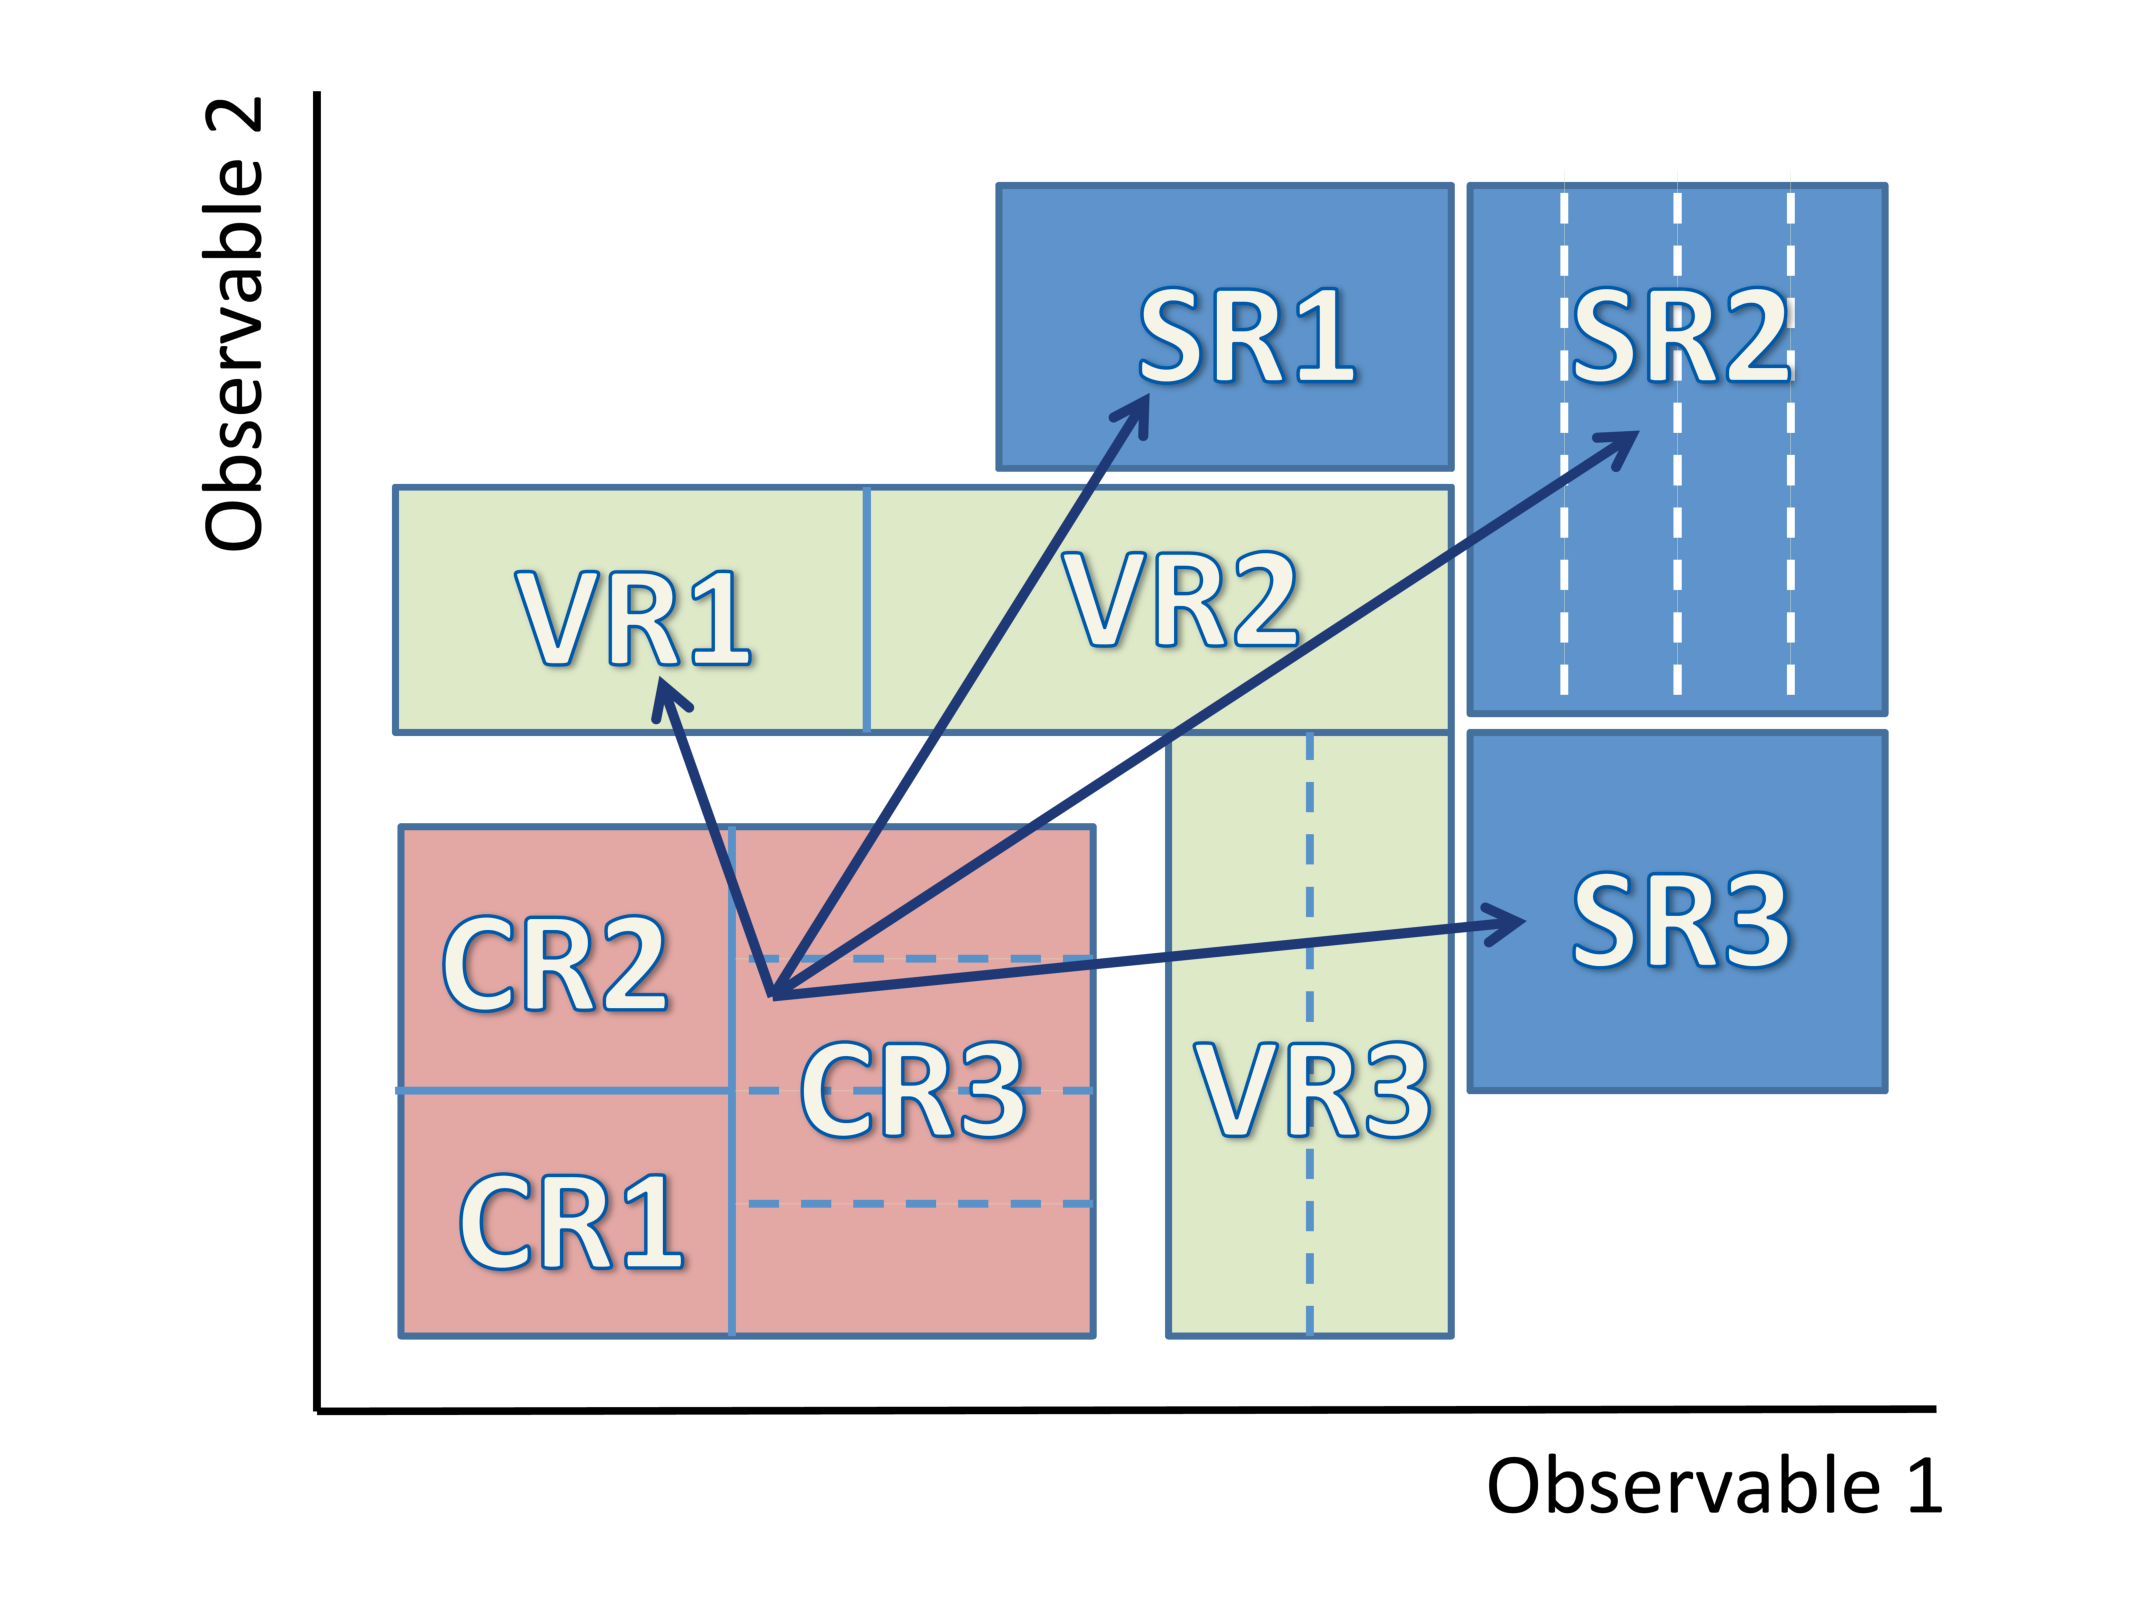
\includegraphics[width=0.65\textwidth]{./figures/statistics/CR_VR_SR.pdf}
\caption{\label{fig:CR_VR_SR_stat}{Basic diagram of data driven background estimation techniques.  We define control regions (CR) that is dominated by background and have little signal.  We can estimate the amount of background we expect in the signal region (SR) by measuring the amount of background in the CR and extrapolating to the SR using MC predictions. }}
\end{figure}

\indent If an excess were to exist in the SR, a simultaneous fit to all CR and SR is performed to calculate the statistical significance of any potential excess (discovery fit).   If no excess were found, then a simultaneous fit to all CR and SR is also performed quantify the maximum amount of signal cross-section that can be excluded (exclusion fit).  \\

\indent We also quantify the expected background rate and the systematic uncertainty in SR by performing a background only fit.  In this case, only the CRs are fitted and the SR acts like another VR, receiving the fitted background normalization but not participating in the fit.  The background only fit may give a different predicted background rate from the exclusion or discovery fit because the SR is not simultaneously fitted.  However, the difference is expected to be small because the CRs are designed to have much greater constraining power on background rates then SR.  \\

\indent These three type of fits, the background only fit, the discovery fit and the exclusion fit are covered in more detail in sections \ref{sec:stat:bkgonly} to \ref{sec:stat:limit}. The parameterization of systematics as constrained nuisance parameters is covered in section \ref{sec:stat:sys}. \\

\indent We use the software package $\HistFitter$ (version {\tt HistFitter-00-00-53} ) to perform the statistical analysis.\cite{HistFitter}  At its core $\HistFitter$ is still performing log likelihood fitting based on the principle introduced in section \ref{sec:stat:likelihood} but \HistFitter provide many tools to easily manage and integrate multiple CR, VR, SR, signal samples, backgrounds, and systematics.  $\HistFitter$ is built upon other statistical analysis software including \RooFit.\cite{RooFit}

\section{Parameterization of Systematics as Gaussian Constraints}
\label{sec:stat:sys}

\indent Systematics uncertainties are parameterized as fitted parameters called nuisance parameters.  In general, the nuisance parameter $\alpha$, is constrained to a particular value by a constraint function $C(\alpha)$.   The constraint function $C(\alpha)$ is multiplied to the likelihood as shown in equation \ref{eqn:stat:sys} and contributes to the total likelihood.  The fitted PDF $P(x|\vec{z},\alpha)$ can depend on a number of unconstrained fitted parameter $\vec{z}$ and the constrained $\alpha$.  

\begin{equation}
\label{eqn:stat:sys}
{\mathcal{L}}(\vec{z},\alpha) = {\displaystyle\prod_{i=1}^{n}} P(x_i|\vec{z},\alpha) C(\alpha)
\end{equation}

%\indent Now the value of $\alpha$ corresponding to the maximum likelihood ${\mathcal{L}}(\vec{z},\alpha)$ may not be the same as value where $C(\alpha)$ is maximized.  Depending on the data points $x_i$, the component of the likelihood from ${\displaystyle\prod_{i=1}^{n}} P(x_i|\vec{z},\alpha)$ maybe bigger even if $C(\alpha)$ is not at its maximum. \\

\indent We pay a penalty on the total likelihood if the nuisance parameter $\alpha$ deviates from the value with maximum $C(\alpha)$.  The fit finds the optimal point between changing the $\alpha$ so that the PDF best describes the data and the cost from the constraint function on $\alpha$. \\

\indent We use Gaussians as the constraint function for all systematics.  The nominal value corresponds to $\alpha = 0$ and the plus and minus $1\sigma$ deviation corresponds to $\alpha = \pm1$.  \\

%\indent Two types of systematics exist  for our analysis; normalization and shape systematics.  Normalizations systematics are only applied to the total background and signal rate in the SR. On the other hand, shape systematics the PDF shape to differ.  Therefore, a shape systematic can affect different $\RISR$ bin differently in SR.  \\

\section{Background Only Fit and Background Estimation}
\label{sec:stat:bkgonly}

\indent The background rates are normalized to data through a simultaneous fit to CRs for the background only fit.  The fitted background normalizations derived from the fit are then applied to the SR but the SR is not simultaneously fitted.  No signal sample is included in the fit and any potential signal contamination in the CR is ignored.  This fit has the advantage of being able to quantify the expected background rate and systematic uncertainties while the SR is blinded. \\

%The background only fit is performed to estimate the background systematic uncertainties and the expected background rate in SR.  \\

\indent The background normalizations predicted in the background only fit may differ from the discovery and exclusion fits because the SR is simultaneously fitted in those fits. This difference should be small as long as the CRs have high background purity and significantly higher statistics then SR.  \\

\section{Exclusion Fit and Exclusion Limit Calculation}
\label{sec:stat:limit}

\indent The exclusion fit is performed as a simultaneous fit to all CRs and all five SR $\RISR$ bins. The signal sample is included in both CR and SR and normalized to the fitted signal strength parameter.   \\

\indent The best fit signal strength is found when the negative log likelihood (NLL) is at a minimum after fitting to data.  As the signal strength deviates from the best fit value, the NLL increases and we are more confident that the signal strength is not supported by data.  We use the difference in NLL as our test statistic.  The relationship between the test statistic and statistical significance is approximated by a parabola in the asymptotic high statistics case. \\

\indent We can calculate the NLL corresponding to the nominal signal strength of each signal model and compare it with the fitted minimum NLL.  The difference in the two NLLs can be converted into the statistical significance using the parabolic relationship between the two.  The statistical significance is quantified as the exclusion confidence limit (CL$_s$).  If the CL$_s$ is below 5 percent then the signal model has been excluded to 95 confidence. \\

\indent We calculate the CL$_s$ corresponding to a grid of signal models each with a different stop and neutralino mass.  The CL$_s$ are plotted in a 2D graph with the stop mass along the x-axis and the neutralino mass along the y-axis.  These CL$_s$ are then interpolated over to form a 2D contour plot.  The contour corresponding to the 95 percent CL$_s$ defines the parameter space excluded by the search. \\

\indent We can also find the 95 percent confidence limit on the observed signal cross-section in each $\RISR$ bin.  The observed signal cross-section is defined as the number of signal events predicted to exist in SR for any particular signal model and is equivalent to selection efficiency times the signal production cross-section.  The limit on the observed cross-section is completely theory independent.  It is simply a statement on the maximum additional BSM rate that can exist in SR without being ruled out to 95 percent confidence.  \\

\section{Discovery Fit and Discovery Significance Calculation}
\label{sec:stat:discovery}

\indent The discovery fit is also performed as a simultaneous fit to all CRs and SR.  The signal sample is included only in the SR but not to the CR in the fit.  Excluding the signal sample from the CR gives a more conservative estimate.  If a signal is present in nature, the signal contamination would still contribute to the CR yield in data.  The higher data yield will in turn increase background normalizations in CR.  Hence, any potential signal contamination is considered essentially as additional background in CR. \\

\indent  Again, a well designed CR has little signal contamination so the difference between this approach and exclusion fit should be small.  Our signal contamination is less then 12 percent for all relevant signal samples.  The signal contamination drops to below 10 percent for all stop masses above 300 GeV.  \\  

\indent We do not statically combine the 5 $\RISR$ bins for the discovery fit.  The single $\RISR$ bin with the best significance is used to calculate the discovery significance.  Again this is a conservative approach and gives us worse discovery significances but it makes the analysis less sensitive to potential shape uncertainties in signal.  \\

\indent We also use the difference in NLL as our test static for our discovery fit.  The signal strength and background normalization that best fit the data is found at the minimum NLL.  Then we calculate the NLL with a signal strength of zero.  The difference between the zero signal strength NLL and the best fit NLL is our test statistic.  The relationship between the test statistic and statistical significance is given by a parabola in the asymptotic high statistics case. \\%We assume we are in the asymptotic case and derive the statistic significance of the zero signal strength fit.  \\

\indent The statistical significance of the zero signal strength fit is the p-value of the no signal hypothesis test.  This p-value quantifies the discovery significance for the analysis.  If the discovery significance is above 5 sigma then discovery can be claimed.\\

